\documentclass[14pt]{extarticle}
\input{external/preamble-latex-cools.tex}
\begin{document}
\begin{project}{Actividad de cierre}{Los globos de Andre.}{cool-globosGruposIguales}%
Andre tenía 125 globos. Él y 4 amigos colgaron algunos de esos globos para una fiesta en la escuela y ahora quedan 80 globos. Si cada persona colgó el mismo número de globos, ¿cuántos globos colgó cada uno?%
%
\begin{enumerate}[label={(\alph*)}]
\item{}Escribe una ecuación que corresponda a la situación y que tenga una letra para representar la cantidad desconocida.%
\begin{image}{0}{1}{0}{}%
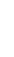
\includegraphics[max width=\linewidth, center]{external/whitespace-tikz/1cm.pdf}
\end{image}%
\item{}Resuelve el problema. Explica o muestra cómo razonaste.%
\begin{image}{0}{1}{0}{}%
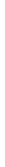
\includegraphics[max width=\linewidth, center]{external/whitespace-tikz/4cm.pdf}
\end{image}%
\end{enumerate}
\end{project}
\end{document}